\section{连续映射}
\label{sec:topo-continuous-maps}

前两节研究一个空间内部的子集与点列，本节转向两个空间之间的映射。实函数$f$在$x_0$处连续的含义是：只要输入留在$x_0$附近某个足够小的区间内，输出就留在$f(x_0)$附近指定的区间内。这个要求可以改用开集表达，从而推广到任意拓扑空间。

\subsection{连续性的定义}
\label{sec:topo-continuity-definition}

先看$\varepsilon$-$\delta$定义在说什么。给定连续的$f:\mathbb R\to\mathbb R$及开集$V\subseteq\mathbb R$，设$f(x_0)\in V$，取$\varepsilon$使$(f(x_0)-\varepsilon,f(x_0)+\varepsilon)\subseteq V$。连续性给出$\delta>0$，使
\[
 (x_0-\delta,x_0+\delta)\subseteq f^{-1}(V).
\]
这对$f^{-1}(V)$的每个点成立，所以$f^{-1}(V)$是开集。逐点的“输入附近映入输出附近”就这样变成了一句关于原像的话。

图~\ref{fig:topo-preimage}(a)取$f(x)=x^2$，$V=(1,4)$，解$1<x^2<4$得
\[
 f^{-1}(V)=(-2,-1)\cup(1,2),
\]
这是开集。在点$x_0=3/2$处，$(1,2)$就是一个可用的区间，对应$\delta=1/2$。

图~\ref{fig:topo-preimage}(b)是有跳跃的函数，$x<1$时$f(x)=x$，$x\geq1$时$f(x)=x+1$。取$V=(3/2,5/2)$，$x<1$的部分取值小于$1$，不进入$V$；$x\geq1$的部分要求$x+1<5/2$。于是
\[
 f^{-1}(V)=[1,3/2),
\]
它含左端点而在那里没有余地，不是开集。跳跃恰好表现为某个开集的原像不开。

\begin{BookInlineFigure}
  \centering
  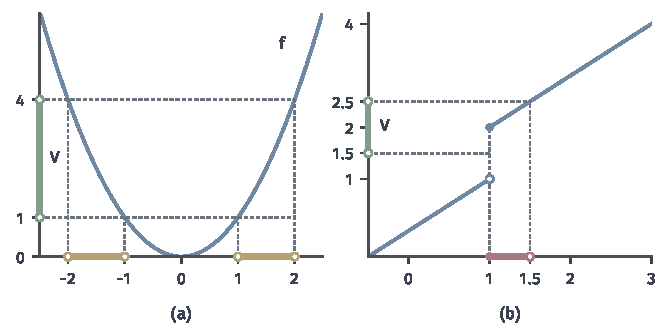
\includegraphics[width=112mm]{figures/04-spaces-measures-and-geometry/01-topology-and-metric/matplotlib/topo-preimage/figure.pdf}
  \caption{开集的原像。绿色是纵轴上的开区间$V$。(a)$f(x)=x^2$，$V=(1,4)$的原像是横轴上的$(-2,-1)\cup(1,2)$（黄色），仍是开集。(b)$f$在$x=1$处跳跃，$V=(3/2,5/2)$的原像是$[1,3/2)$（红色），含端点$1$，不是开集。}
  \label{fig:topo-preimage}
\end{BookInlineFigure}

\begin{definition}[连续映射]
\label{def:topo-continuous-map}
设$X,Y$是拓扑空间。映射$f:X\to Y$称为\term{连续映射}（continuous map），如果对$Y$的每个开集$V$，下面的原像都是$X$的开集：
\begin{equation}
 f^{-1}(V)=\{x\in X:f(x)\in V\}.
 \label{eq:topo-preimage}
\end{equation}
\end{definition}

定义用原像，是因为原像与集合运算相容：
\[
\begin{gathered}
 f^{-1}\Bigl(\bigcup_iV_i\Bigr)=\bigcup_if^{-1}(V_i),\qquad
 f^{-1}\Bigl(\bigcap_iV_i\Bigr)=\bigcap_if^{-1}(V_i),\\
 f^{-1}(Y\setminus V)=X\setminus f^{-1}(V).
\end{gathered}
\]
这些等式可参考\BookChapterRef{chap:sets-relations-maps}{卷一第1章“集合、关系与映射”}。由第一个等式，若$\mathcal B$是$Y$的拓扑基，只需检验每个$B\in\mathcal B$的原像为开集，因为任意开集都是基本开集之并。

\paragraph{等价判据}
定义~\ref{def:topo-continuous-map}是整体的说法。处理具体映射时，有时逐点检验更方便，有时检验闭集更方便。

\begin{theorem}[连续性的等价刻画]
\label{thm:topo-continuity-equivalent}
对映射$f:X\to Y$，下列条件等价：
\begin{enumerate}
  \item $f$连续；
  \item 对每个$x\in X$及$f(x)$的每个邻域$V$，存在$x$的邻域$U$使$f(U)\subseteq V$；
  \item 对$Y$的每个闭集$F$，$f^{-1}(F)$是$X$的闭集。
\end{enumerate}
\end{theorem}
\begin{proof}
1推出2。$V$含开集$V'\ni f(x)$，$U=f^{-1}(V')$是含$x$的开集，并且$f(U)\subseteq V'\subseteq V$。

2推出1。设$V$开，$x\in f^{-1}(V)$。$V$是$f(x)$的邻域，取$x$的邻域$U$使$f(U)\subseteq V$，则$U\subseteq f^{-1}(V)$。所以$f^{-1}(V)$是它每个点的邻域，由引理~\ref{lem:topo-open-iff-neighborhood}是开集。

1与3的等价来自等式$f^{-1}(Y\setminus F)=X\setminus f^{-1}(F)$：闭集的补集是开集，原像的补集是补集的原像。
\end{proof}

条件2在$X=Y=\mathbb R$时取邻域基$(x-\delta,x+\delta)$与$(f(x)-\varepsilon,f(x)+\varepsilon)$，就是$\varepsilon$-$\delta$定义，所以通常拓扑下的连续与卷一的连续一致。常值映射总是连续的，因为任何集合的原像只能是$\varnothing$或$X$。

\begin{example}[连续性依赖两边的拓扑]
\label{ex:topo-continuity-depends-topology}
考虑恒等映射$\operatorname{id}:\mathbb R\to\mathbb R$。若定义域取离散拓扑，则无论值域取什么拓扑，它都连续，因为定义域的每个子集都开。

若定义域取通常拓扑、值域取离散拓扑，则$\{0\}$在值域中开，原像$\{0\}$在定义域中不开，恒等映射不连续。同一个集合映射，连续与否由两边的开集族共同决定。
\end{example}

\paragraph{复合与点列}
连续映射的复合仍然连续。设$f:X\to Y$与$g:Y\to Z$连续，$W$是$Z$的开集，则
\[
 (g\circ f)^{-1}(W)=f^{-1}\bigl(g^{-1}(W)\bigr).
\]
先由$g$连续得到$g^{-1}(W)$开，再由$f$连续得到它的原像开。连续映射也保持已有的点列极限。

\begin{theorem}[连续映射保持极限]
\label{thm:topo-continuous-preserves-limits}
设$f:X\to Y$连续，$X$中的点列$x_n\to x$，则$f(x_n)\to f(x)$。
\end{theorem}
\begin{proof}
设$V$是$f(x)$的邻域。由定理~\ref{thm:topo-continuity-equivalent}，有$x$的邻域$U$使$f(U)\subseteq V$。由$x_n\to x$，$n$充分大时$x_n\in U$，于是$f(x_n)\in V$。
\end{proof}

反过来，“保持所有收敛点列的极限”能否推出连续，取决于点列能否探测定义域的拓扑。在余可数拓扑（例~\ref{ex:topo-cocountable}）中只有最终恒定的点列收敛，所以从这个空间出发的任何映射都保持极限。

然而从余可数拓扑的$\mathbb R$到通常拓扑的$\mathbb R$的恒等映射并不连续：开集$(0,1)$的补集不可数，原像$(0,1)$不是余可数拓扑的开集。在度量空间中，序列判据与连续性等价，这在第~\ref{chap:metric-space-maps}章证明。

\paragraph{原像与像}
连续性约束的是原像，对像没有直接约束。连续映射$f(x)=x^2$把开区间$(-1,1)$映成$[0,1)$，见图~\ref{fig:topo-image-openness}(a)，它不是开集。连续映射$g(x)=\arctan x$把闭集$\mathbb R$映成$(-\pi/2,\pi/2)$，它不是闭集。

像对集合运算的行为也不如原像整齐：像与并相容，但$f(A\cap B)$一般只包含于$f(A)\cap f(B)$。取$f(x)=x^2$，$A=\{-1\}$，$B=\{1\}$，则
\[
 f(A\cap B)=\varnothing,\qquad f(A)\cap f(B)=\{1\}.
\]

\subsection{开映射}
\label{sec:topo-open-maps}

上一小节的例子提出另一个问题：哪些映射把开集映成开集？这个条件与连续性平行，方向却相反。

\begin{definition}[开映射]
\label{def:topo-open-map}
映射$f:X\to Y$称为\term{开映射}（open map），如果对$X$的每个开集$U$，像$f(U)$是$Y$的开集。
\end{definition}

由于$f(\bigcup_iU_i)=\bigcup_if(U_i)$，验证开映射只需对定义域的某个拓扑基检验。

两个条件互不蕴含。常值映射$f(x)=c$连续，但$f((0,1))=\{c\}$不是开集，所以连续不保证开映射。反过来，从通常拓扑到离散拓扑的恒等映射（例~\ref{ex:topo-continuity-depends-topology}）把每个集合映成离散拓扑中的开集，是开映射，却不连续。

开映射的典型例子是平面到坐标轴的投影$p(x_1,x_2)=x_1$。开矩形$(a_1,b_1)\times(a_2,b_2)$的像是$(a_1,b_1)$，而开矩形构成拓扑基，所以$p$是开映射，见图~\ref{fig:topo-image-openness}(b)。

开映射也不必把闭集映成闭集。双曲线$\{(x_1,x_2):x_1x_2=1\}$是连续函数$x_1x_2$在闭集$\{1\}$上的原像，因而闭，它在$p$下的像却是$\mathbb R\setminus\{0\}$，见图~\ref{fig:topo-image-openness}(c)。这个像不含$0$，而$0$是它的闭包点，所以不闭。

\begin{BookInlineFigure}
  \centering
  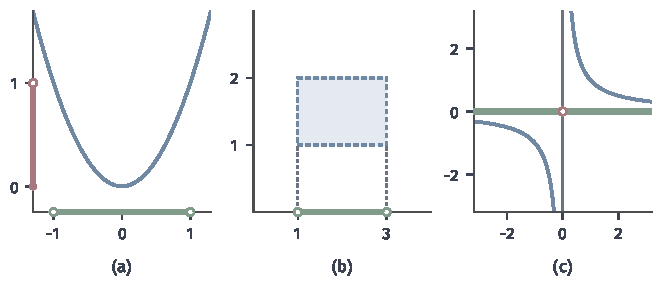
\includegraphics[width=112mm]{figures/04-spaces-measures-and-geometry/01-topology-and-metric/matplotlib/topo-image-openness/figure.pdf}
  \caption{像的开闭性。(a)$f(x)=x^2$把绿色开区间$(-1,1)$映成纵轴上的$[0,1)$（红色），连续而不开。(b)投影把开矩形$(1,3)\times(1,2)$映成开区间$(1,3)$。(c)闭集$x_1x_2=1$在投影下的像是绿色的$\mathbb R\setminus\{0\}$，缺少原点，不闭。}
  \label{fig:topo-image-openness}
\end{BookInlineFigure}

\subsection{同胚}
\label{sec:topo-homeomorphisms}

两个拓扑空间什么时候应当看作“相同”？线性代数中，可逆线性映射把一边的线性结构原样搬到另一边，于是两个同构的线性空间不必区分。拓扑中的对应角色是：一个双射把一边的开集恰好对应到另一边的开集。这时一切只用开集表述的概念（邻域、闭包、收敛、连续）都会被这个双射原样搬过去。

\begin{definition}[同胚]
\label{def:topo-homeomorphism}
双射$f:X\to Y$称为\term{同胚}（homeomorphism），如果$f$与逆映射$f^{-1}$都连续。存在同胚时，称$X$与$Y$同胚，记作$X\cong Y$。
\end{definition}

$f$连续说明$Y$的开集对应到$X$的开集。$f^{-1}$连续说明$X$的开集$U$的像$f(U)=(f^{-1})^{-1}(U)$是$Y$的开集。所以同胚在两边的开集族之间建立了一一对应，$x$的邻域也恰好对应到$f(x)$的邻域。

\begin{theorem}[连续双射成为同胚的条件]
\label{thm:topo-homeomorphism-open}
设$f:X\to Y$是连续双射。$f$是同胚，当且仅当$f$是开映射。
\end{theorem}
\begin{proof}
对$X$的开集$U$，$f$是双射，所以
\[
 (f^{-1})^{-1}(U)=\{y:f^{-1}(y)\in U\}=f(U).
\]
于是“$f^{-1}$连续”逐字等于“$f$把每个开集映成开集”。
\end{proof}

连续双射未必是同胚。例~\ref{ex:topo-continuity-depends-topology}中从离散拓扑到通常拓扑的恒等映射是连续双射，但不是开映射，因为$\{0\}$的像不开。第~\ref{sec:topo-subspaces}小节还会给出一个更直观的例子：把半开区间绕成圆周的映射。

\paragraph{同胚不保持长度}
同胚只要求开集对应，不要求保持距离、长度或有界性。仿射映射$x\mapsto a+(b-a)x$是$(0,1)$到$(a,b)$的同胚，它把长度伸缩了$b-a$倍。更进一步，映射
\begin{equation}
 h:(-1,1)\to\mathbb R,\qquad h(x)=\frac{x}{1-\lvert x\rvert}
 \label{eq:topo-interval-line-homeomorphism}
\end{equation}
把有界区间变成整条实轴。

它的逆映射是$h^{-1}(y)=y/(1+\lvert y\rvert)$。验证一下，设$y\geq0$，$x=y/(1+y)$，则$1-\lvert x\rvert=1/(1+y)$，于是
\[
 h(x)=\frac{y/(1+y)}{1/(1+y)}=y.
\]
$y<0$时由$h$是奇函数得到同样的结论。$h$与$h^{-1}$都由连续函数作除法得到，分母不为零，所以都连续。

在具体的点上，$h(1/2)=1$，$h(3/4)=3$，图~\ref{fig:topo-homeomorphism}(a)标出了这些点。输入越靠近$\pm1$，输出越大，距离被任意放大，开集的对应却没有被破坏。

\begin{BookInlineFigure}
  \centering
  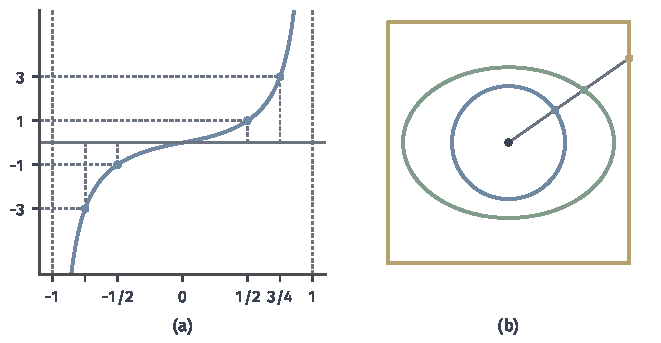
\includegraphics[width=112mm]{figures/04-spaces-measures-and-geometry/01-topology-and-metric/matplotlib/topo-homeomorphism/figure.pdf}
  \caption{同胚不保持度量性质。(a)$h(x)=x/(1-\lvert x\rvert)$把$(-1,1)$连续地拉成整条实轴，图中标出了$\pm1/2$与$\pm3/4$的函数值$\pm1$与$\pm3$。(b)从中心出发的射线与圆周、椭圆、正方形边界各交一点，沿射线移动这些交点就得到三条曲线之间的同胚。}
  \label{fig:topo-homeomorphism}
\end{BookInlineFigure}

有界性、长度都不是拓扑性质。拓扑性质指同胚保持的性质，例如本章后面的连通性与紧性。

同样，平面上的单位圆周与正方形边界同胚，这里的正方形边界是
\[
 \{\bm y:\max(\lvert y_1\rvert,\lvert y_2\rvert)=1\}.
\]
从原点出发的每条射线与两条曲线各交于一点，沿射线移动的映射是
\[
 F(\bm x)=\frac{\bm x}{\max(\lvert x_1\rvert,\lvert x_2\rvert)},\qquad
 F^{-1}(\bm y)=\frac{\bm y}{\sqrt{y_1^2+y_2^2}}.
\]

取$\bm x=(3/5,4/5)$，除以$4/5$得$F(\bm x)=(3/4,1)$；再除以其长度$5/4$，回到$(3/5,4/5)$。图~\ref{fig:topo-homeomorphism}(b)还画了椭圆，同样的射线也给出它与另外两条曲线的对应。三者周长和弯曲程度各不相同，拓扑只记录它们首尾相接成一圈的结构。要严格核对这类平面子集上的开集，需要下一节的子空间拓扑。
